\documentclass{standalone}
\usepackage{hsbcommon}
\makeatletter\AtBeginDocument{\@buildstepset{1,2,3,4,5}}\makeatother
\begin{document}
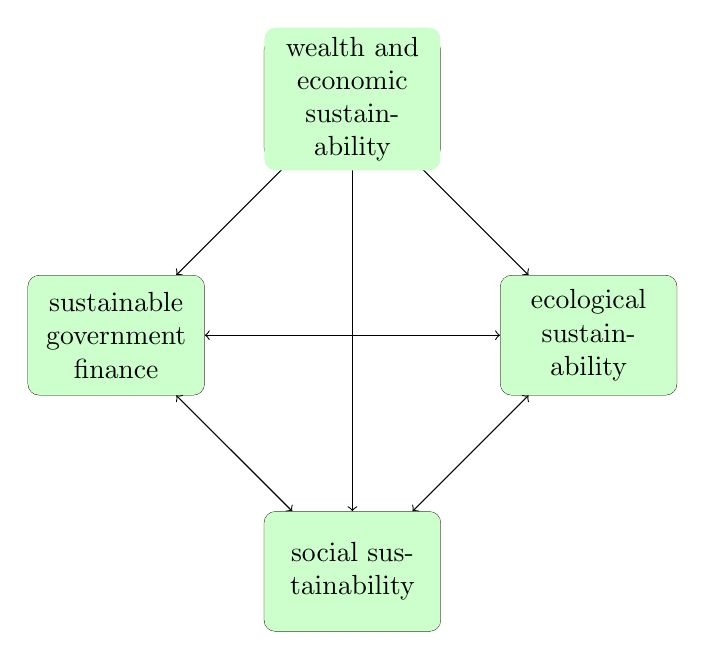
\begin{tikzpicture}
    \tikzset{
        goal/.style={
            draw,
            text width=2cm,
            minimum height=10ex,
            align=center,
            rounded corners
        }
    }
    \foreach [count=\i] \myziel in 
    {%
    full employment,
    stable price level,
    economic growth,
    external economic equilibrium%
    }
    {
        \node[goal] (N\i) at (90*\i:3) {};
    }
    \foreach \i in {1,2,3,4}
    \foreach \ii in {\i,...,4}
        {\ifnum\i=\ii\else
        \draw[<->] (N\i) -- (N\ii);
        \fi}

    \ifstep{1}{
        \foreach [count=\i] \myziel in 
            {%
            full employment,
            stable price level,
            economic growth,
            external economic equilibrium%
            }
            {
                \node[goal, draw=none, fill=yellow!20] (N\i) at (90*\i:3) {\myziel};
            }
    }
    
    \ifstep{2}{
        \foreach [count=\i] \myziel in 
            {%
            wealth and economic sustainability,
            sustainable government finance,
            social sustainability,
            ecological sustainability
            }
            {
                \node[goal, draw=none, fill=green!20] (M\i) at (90*\i:3) {\myziel};
            }    
    }
    
\end{tikzpicture}
\end{document}
